\documentclass[
  10pt, % Fontsize
  a4paper, % papersize
  twoside, % For twosided documents
  openright, % Chapters start always at a odd page
  numbers=noenddot, % No final dots in Sectionnumbers, e.g 1.2 instead of 1.2.
  BCOR=5mm, % Correction length for lost space from binding
  parskip=half*, %No indent but spacing between paragraphs
  thesis, % type of document
]{bfhbook}


% Test Template for bfhbook.cls
\usepackage[T1]{fontenc}
% Coding 
\usepackage[utf8]{inputenc}
% Language setting
\usepackage[german]{babel}
\usepackage[export]{adjustbox}

% \usepackage{fonttable}
% Hyperref
\usepackage[                
  pdftex,                  % for PDF
  colorlinks=true,         % colored links
  linkcolor=black,         % color for links
  citecolor=black,         % color for references
  urlcolor=black,          % color for url 
  bookmarks=true
]{hyperref}              

\usepackage{booktabs} % For nicer tables
\usepackage{threeparttable} % Table-Captions having the same width than the table
\usepackage[singlelinecheck=off]{caption}
\usepackage{siunitx} % Scientific Units and number setting
\usepackage{listings} % For Program-Code
\usepackage{minted}
\usepackage{caption}

\usepackage{glossaries}

%%%%%%%%%%%%%%%%%%%%%%%%%%%%%%%%%%%
% Settings 
%%%%%%%%%%%%%%%%%%%%%%%%%%%%%%%%
% Type?? (Lecture Notes, BSc Thesis, Master Thesis, . . .) 
% Use Variables \BSc, \Master, etc. for language support
\type{Semesterarbeit}
% Author(s)
\author{Marc Habegger}
% Title
\title{IoT Erfassung von und Darstellung Sensordaten}
% Short Title, will be used in the footline
\shorttitle{CAS BGD Semesterarbeit}
% Subtitle
\subtitle{CAS Big Data}
% Titlepicture
\titlepicture{Bilder/Titel.png}
%%

% Topic of Study
\degreeprogramme{Semesterarbeit CAS Big Data}
% Expert
\expert{Max Kleiner}
% Version
\version{1.0}
% Date
\date{\today} % Or any other possible date

% Departement
% Use Variable for language support
%\TI

% Semester
% Use Variable for language support
%\semester

% Logo(s)

% Colors
% Secondary Color for Graphics, Tables etc.
% Naming: BFH*Color*light|middle|dark, e.g. BFHGreendark, BFHBluelight, etc.
% Possible Color Values: Green, Blue, Purple, Brown 
\newcommand{\seccolor}{BFHLightGreen} 

\setcounter{secnumdepth}{4}
\setcounter{tocdepth}{4}

\makeindex
\makeglossaries

\begin{document}
 
\newglossaryentry{IoT}
{
    name=Internet of Things,
    description={deutsch Internet der Dinge, Bezeichnet ein loses Netzwerk in welcher beliebige elektronische Geräte untereinander vernetzt werden. Wir häufig im Zusammenhang mit Sensornetzwerken verwendet.\break 
    \url{https://de.wikipedia.org/wiki/Internet_der_Dinge}}
}

\newglossaryentry{HMAC}
{
    name=Keyed-Hash Message Authentication Code,
    description={Verfahren zur Absicherung von gesendeten Nachrichten welches mit einer Hash-Funktion und einem geheimen Schlüssel arbeitet.\break
    \url{https://de.wikipedia.org/wiki/Keyed-Hash_Message_Authentication_Code}}
}

\maketitle
%**************************************************************************
\frontmatter % preliminary parts

\tableofcontents
\sloppy
%%%%%%%%%%%%%%%%%%%%%%%%
% Introduction
%**************************************************************************
\mainmatter % The main part
%**************************************************************************
%\part{Part One}
\chapter*{Management Summary}

Das Internet der Dinge (\Gls{IoT}) zeichnet sich neben einer allgegenwärtigen Verfügbarkeit von Daten auch durch eine grosse Anzahl der Datenquellen aus. Mit dieser Arbeit soll das Zusammenspiel der verschiedenen Komponenten eines Sensornetzwerkes mit einem Speichersystem und einer grafischen Analyse aufgezeigt werden.

\begin{figure}[htp]
  \begin{center}
    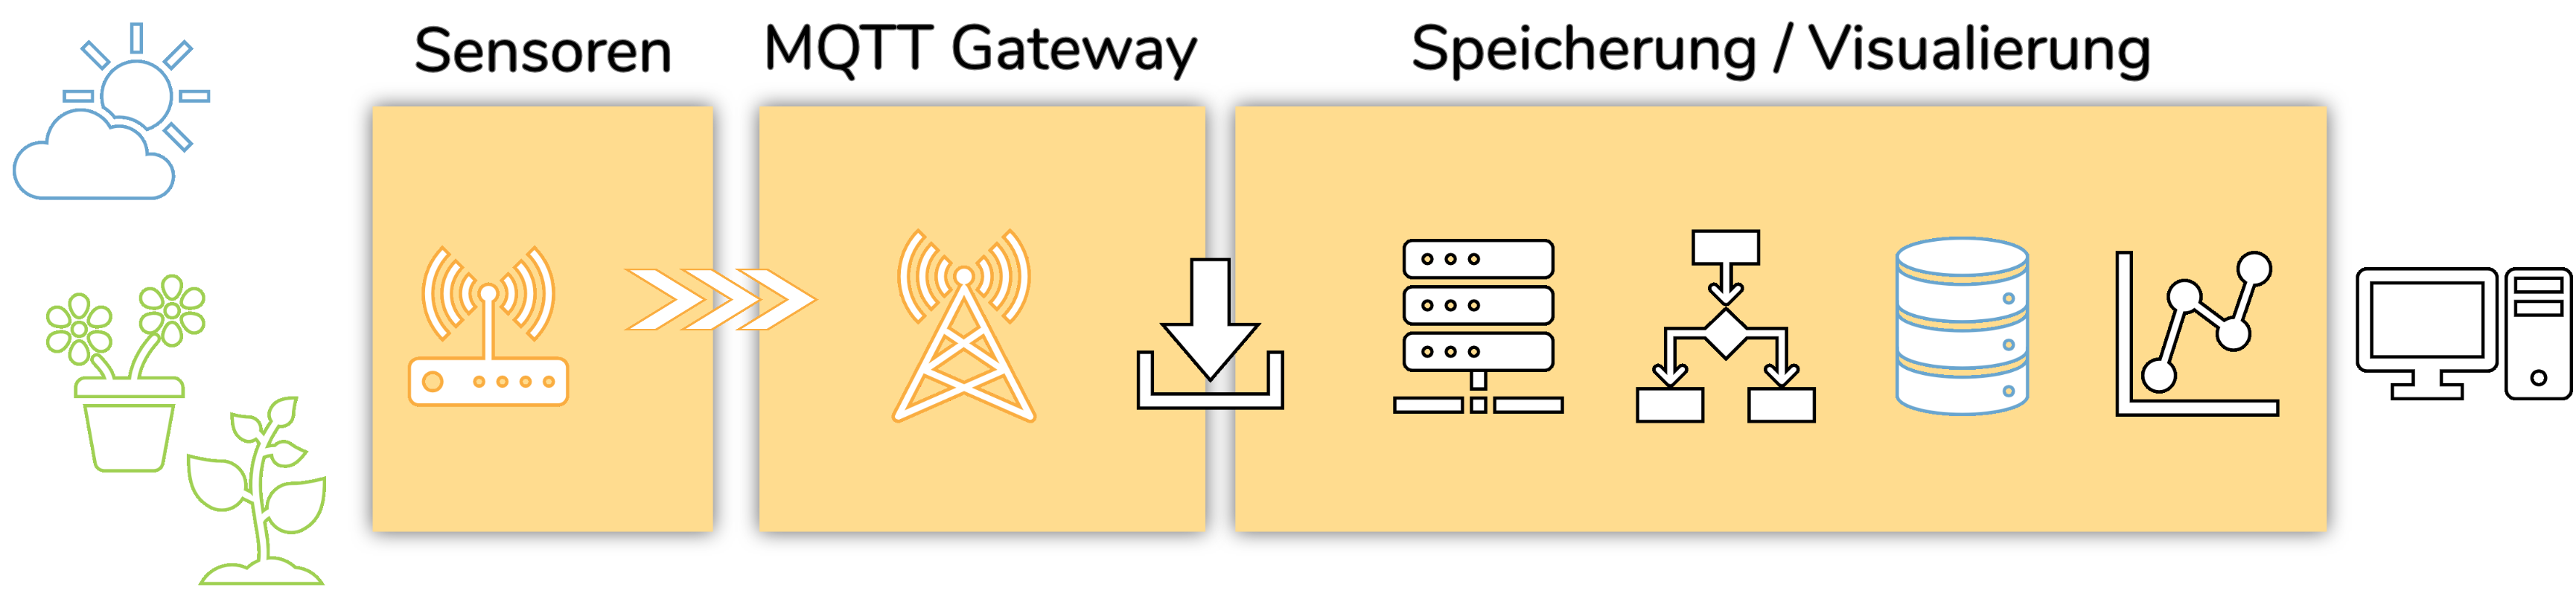
\includegraphics[width=18cm, left]{Bilder/Overview.png}
  \end{center}
    \caption{Systemaufbau}
\end{figure}

\chapter{Einleitung}
\section{Übersicht}
\section{Hardware}
\chapter{Aufbau der Sensoren}
\section{Mikrokontroller}
\begin{figure}[htp]
  \begin{center}
    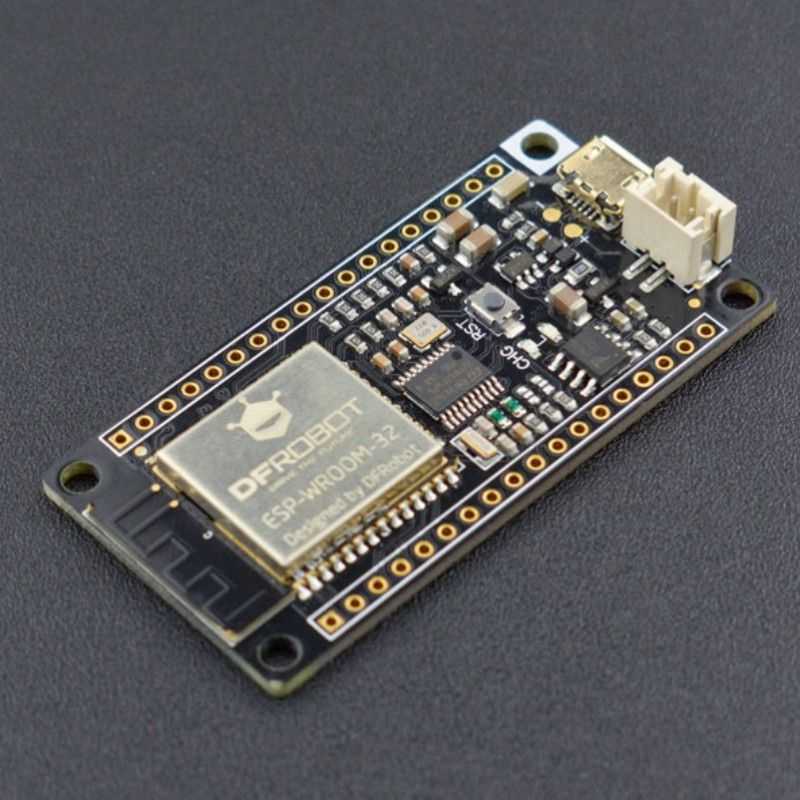
\includegraphics[width=5cm, left]{Bilder/Firebeetle.jpg}
  \end{center}
    \caption{Fireebeetle mit dem ESP32 Mikrokontroller}
  \label{fig:test1}
\end{figure}

 \section{Sensoren}
 \subsection{Temperatur und Luftfeuchtigkeit}
 \subsubsection{DHT22}
 \begin{figure}[htp]
  \begin{center}
    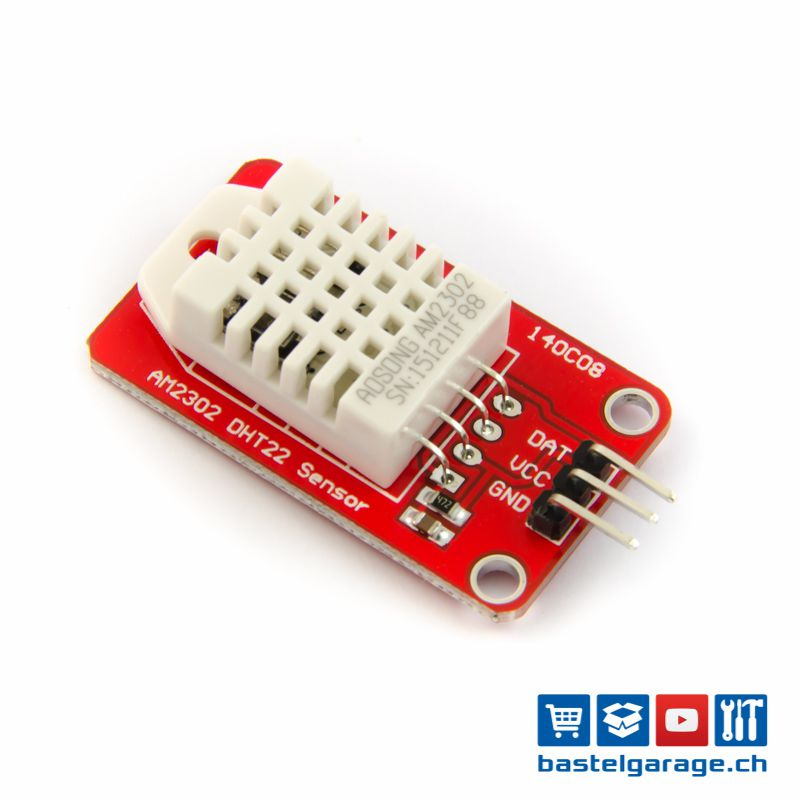
\includegraphics[width=5cm, left]{Bilder/DHT22.jpg}
  \end{center}
    \caption{Temperatur und Luftfeuchtigkeitsmesser DHT22}
  \label{fig:dht22}
\end{figure}
DHT22 im Onlineshop \footnote{https://www.bastelgarage.ch/dht22-temperatur-und-luftfeuchtigkeitssensor-steckbar}
\subsubsection{DHT11}
\subsection{Bodenfeuchtigkeit}

\begin{center}
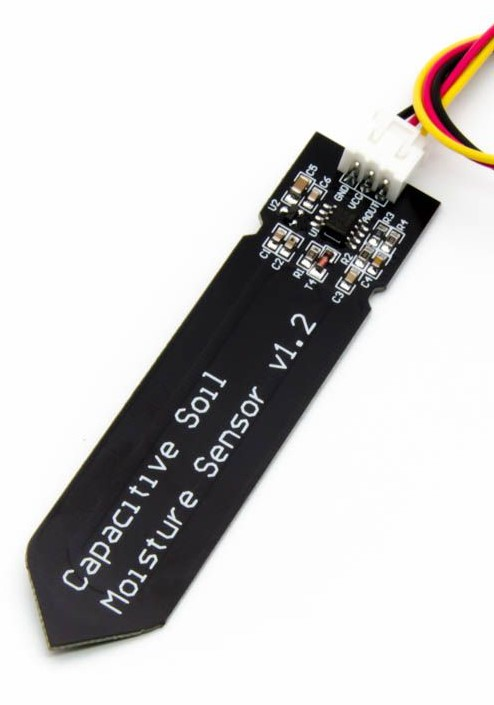
\includegraphics[width=5cm, left]{Bilder/Soil-2.jpg}%
\captionof{figure}{Kapazitiver Bodenfeuchtesensor V1.2}\label{labelname}%
\end{center}
Bodensensor im Onlineshop \footnote{https://www.bastelgarage.ch/bauteile/sensoren/kapazitiver-bodenfeuchtesensor-v1-2}

 \section{Funkverbindung}
 
\begin{center}
    \begin{minipage}[b]{0.45\textwidth}
        \centering
        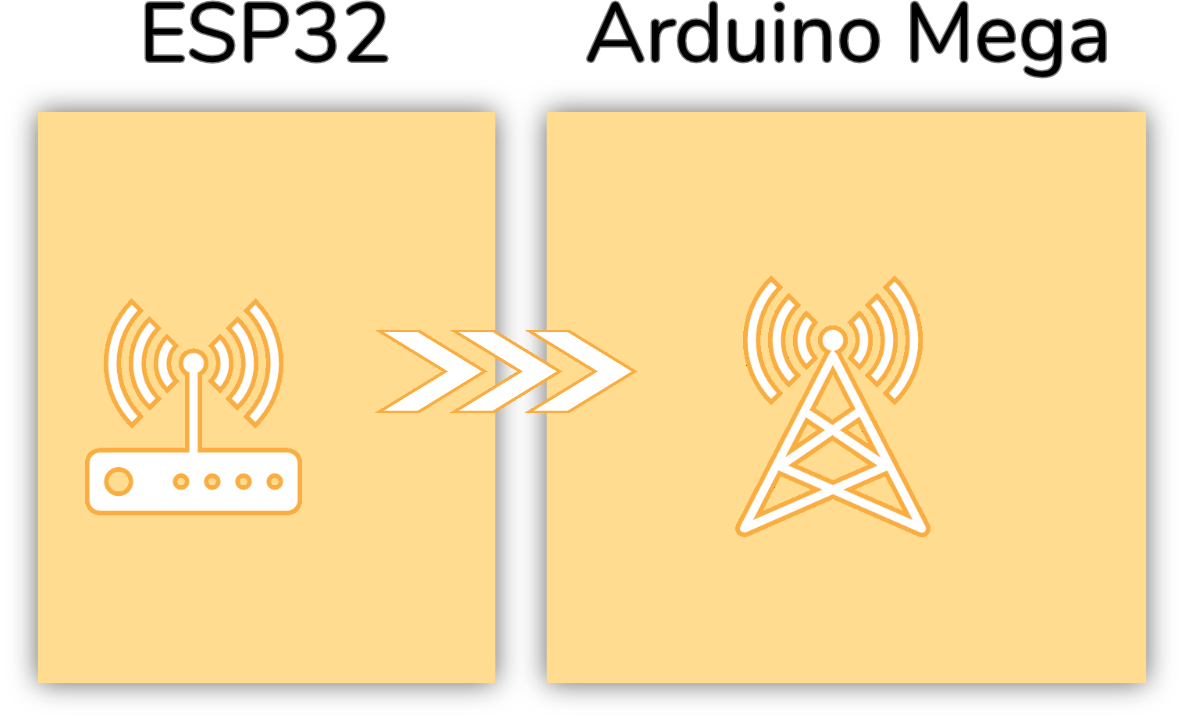
\includegraphics[width=7cm]{Bilder/ESP32-Arduino.png} % first figure itself
        \captionsetup{justification=centering}
        \captionof{figure}{Funkverbindung}
    \end{minipage}\hfill
    \begin{minipage}[b]{0.45\textwidth}
        \centering
        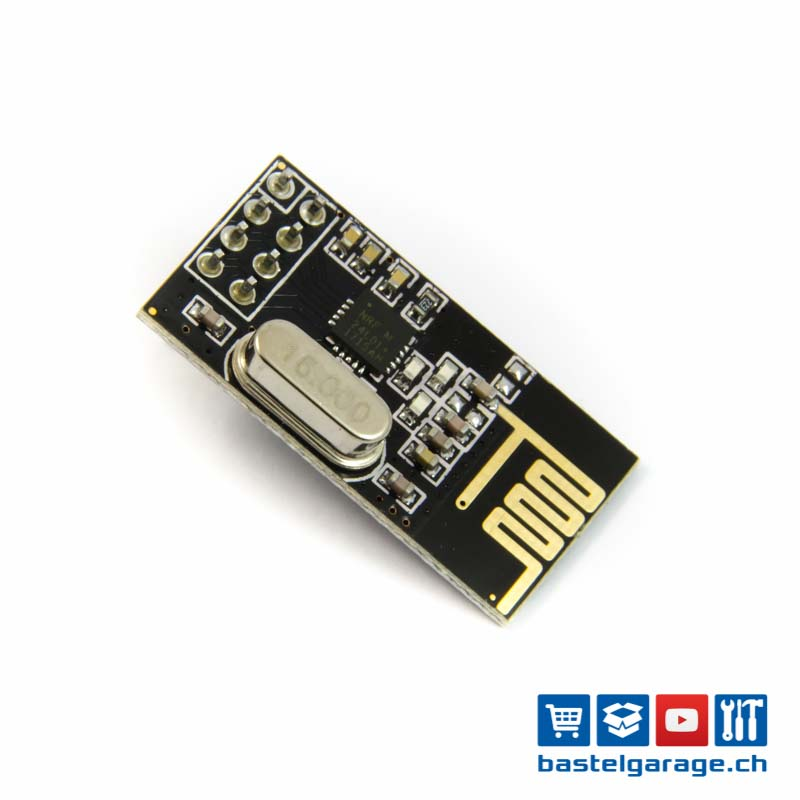
\includegraphics[width=5cm]{Bilder/NRF24.jpg} % second figure itself
        \captionsetup{justification=centering}
        \captionof{figure}{NRF24L01+ Funkmodul}
    \end{minipage}
\end{center}
NRF24L01+ \footnote{https://www.bastelgarage.ch/bauteile/funk-wireless-lora/nrf24l01-wireless-funk-modul-2-4ghz}
 
 \section{Software}

%
\chapter{IoT Gateway}
\section{Übersicht}
\section{Hardware}
\section{Funkverbindung}
\subsection{Zugriffsschutz}
Jede empfangene Nachricht wird durch die Valdierung des HMAC (\Gls{HMAC}) sowohl auf einen berechtigten Absender, als auch auf unverfälschte Daten überprüft.
\section{Software}
\chapter{Speicherung und Visualisierung}
\section{Übersicht}
\begin{center}
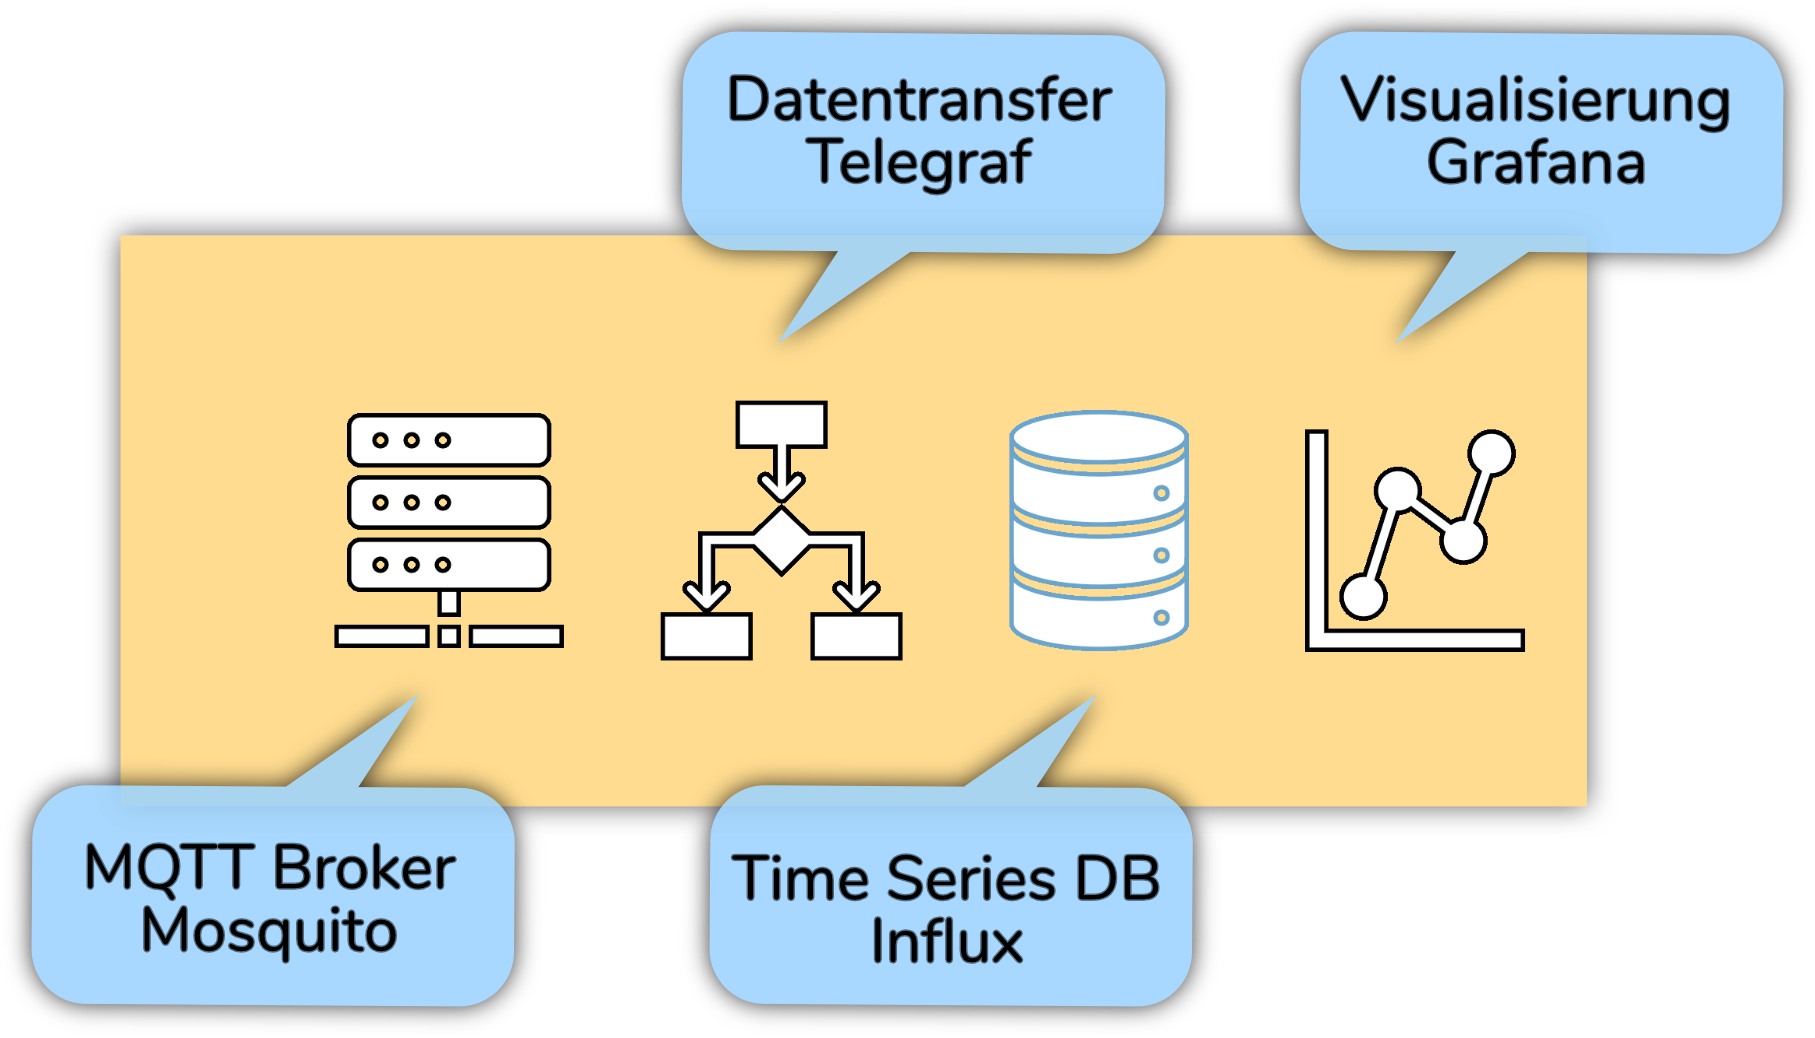
\includegraphics[width=17cm, left]{Bilder/Raspberry-Software.png}%
\captionof{figure}{Verwendete Software}\label{labelname}%
\end{center}
\section{Hardware}
\section{Visualisierung}
\begin{listing}
\begin{minted}[frame=single,
               framesep=3mm,
               linenos=true,
               xleftmargin=21pt,
               tabsize=4]{js}
{     
    "firstName": "John"
    "lastName" : "Smith",
    "age" : 25
}
\end{minted}
\caption{JSON example} 
\label{json-example}
\end{listing}

% List of Figures
\listoffigures
% List of Tables
\listoftables
% Glossary
\printglossary
% Bibliography
\begin{thebibliography}{99}
   \bibitem{whyHmac} What is HMAC Authentication and why is it useful? \url{https://www.wolfe.id.au/2012/10/20/what-is-hmac-authentication-and-why-is-it-useful/}
    \bibitem{esp32-hmac} ESP32 Arduino: Applying the HMAC SHA-256 mechanism \url{https://techtutorialsx.com/2018/01/25/esp32-arduino-applying-the-hmac-sha-256-mechanism/}
    \bibitem{hmacOnline} Online HMAC Code Generator \url{https://www.freeformatter.com/hmac-generator.html#ad-output}
    \bibitem{nrf24} NRF24L01+ Funkmodul Treiber für Arduino und ESP32 \url{http://tmrh20.github.io/RF24/index.html}
    \bibitem{ref4} Dummy entry four.
  \end{thebibliography}
%Index
\addcontentsline{toc}{chapter}{Index}
%\printindex
% Appendices
\end{document}
